\documentclass{beamer}
\usetheme[
  block=fill, 
  background=dark, 
  titleformat=smallcaps,
  progressbar=frametitle,
  numbering=none,
]{metropolis}

%----------------------------------------------------------------------------
% From dyck-paper
%----------------------------------------------------------------------------
\usepackage{caption}
\usepackage{epigraph}
% Math
\usepackage{amsmath}
\usepackage{amssymb}
\usepackage{stmaryrd}
% Code listing
\usepackage{minted}
%\usemintedstyle{friendly}
\usemintedstyle{tango}
\usepackage{algorithm}
\usepackage[noend]{algpseudocode}
% Colors
\usepackage{xcolor}
\colorlet{CodeBg}{gray!90}
\usepackage{color, colortbl}
\definecolor{Gray}{rgb}{0.9,0.9,0.9}
\definecolor{bblue}{HTML}{1D577A}
\definecolor{rred}{HTML}{C03425}
\definecolor{ggreen}{HTML}{8BB523}
\definecolor{ppurple}{HTML}{6B1B7F}
\definecolor{pblack}{HTML}{000000}
\definecolor{pyellow}{HTML}{C0B225}
% Graphs
\usepackage{tikz}
\usetikzlibrary{calc}
\usetikzlibrary{trees}
\usetikzlibrary{positioning}
\usepackage{pgfplots}
% Graphics
\usepackage{graphics}
\graphicspath{{figures/}} % Location of the graphics files

\newcommand\todo[1]{\textcolor{red}{#1}}
\newcommand{\w}[1]{\textit{"#1"}}
\newcommand\s{\textsc}

\newcommand{\Order}[5]{
	\[
	\mathcal{#1}_{#5}\llbracket #2 \leftarrow #3 \mid \{ #4 \} \rrbracket.
	\]
}
\newcommand{\Orderr}[5]{
	\mathcal{#1}_{#5}\llbracket #2 \leftarrow #3 \mid \{ #4 \} \rrbracket.
}
\newcommand{\Ord}[4]{\Order{O}{#1}{#2}{#3}{#4}}
\newcommand{\Or}[4]{\Orderr{O}{#1}{#2}{#3}{#4}}
\newcommand{\Con}[4]{\Order{C}{#1}{#2}{#3}{#4}}
%----------------------------------------------------------------------------

% Beamer
\title{$D^3$ as a 2-MCFL}
\subtitle{}
\author{Orestis Melkonian, Konstantinos Kogkalidis}
\date{January 25, 2018}
\institute{Universiteit Utrecht}

% Box macro
\newcommand{\ex}[2]{
  \vfill
  \begin{alertblock}{#1}
    #2
  \end{alertblock}
}

\begin{document}
	\maketitle
	
	\begin{frame}{}
	\begin{center}
	\vspace{1cm}
	\colorbox{white}{
    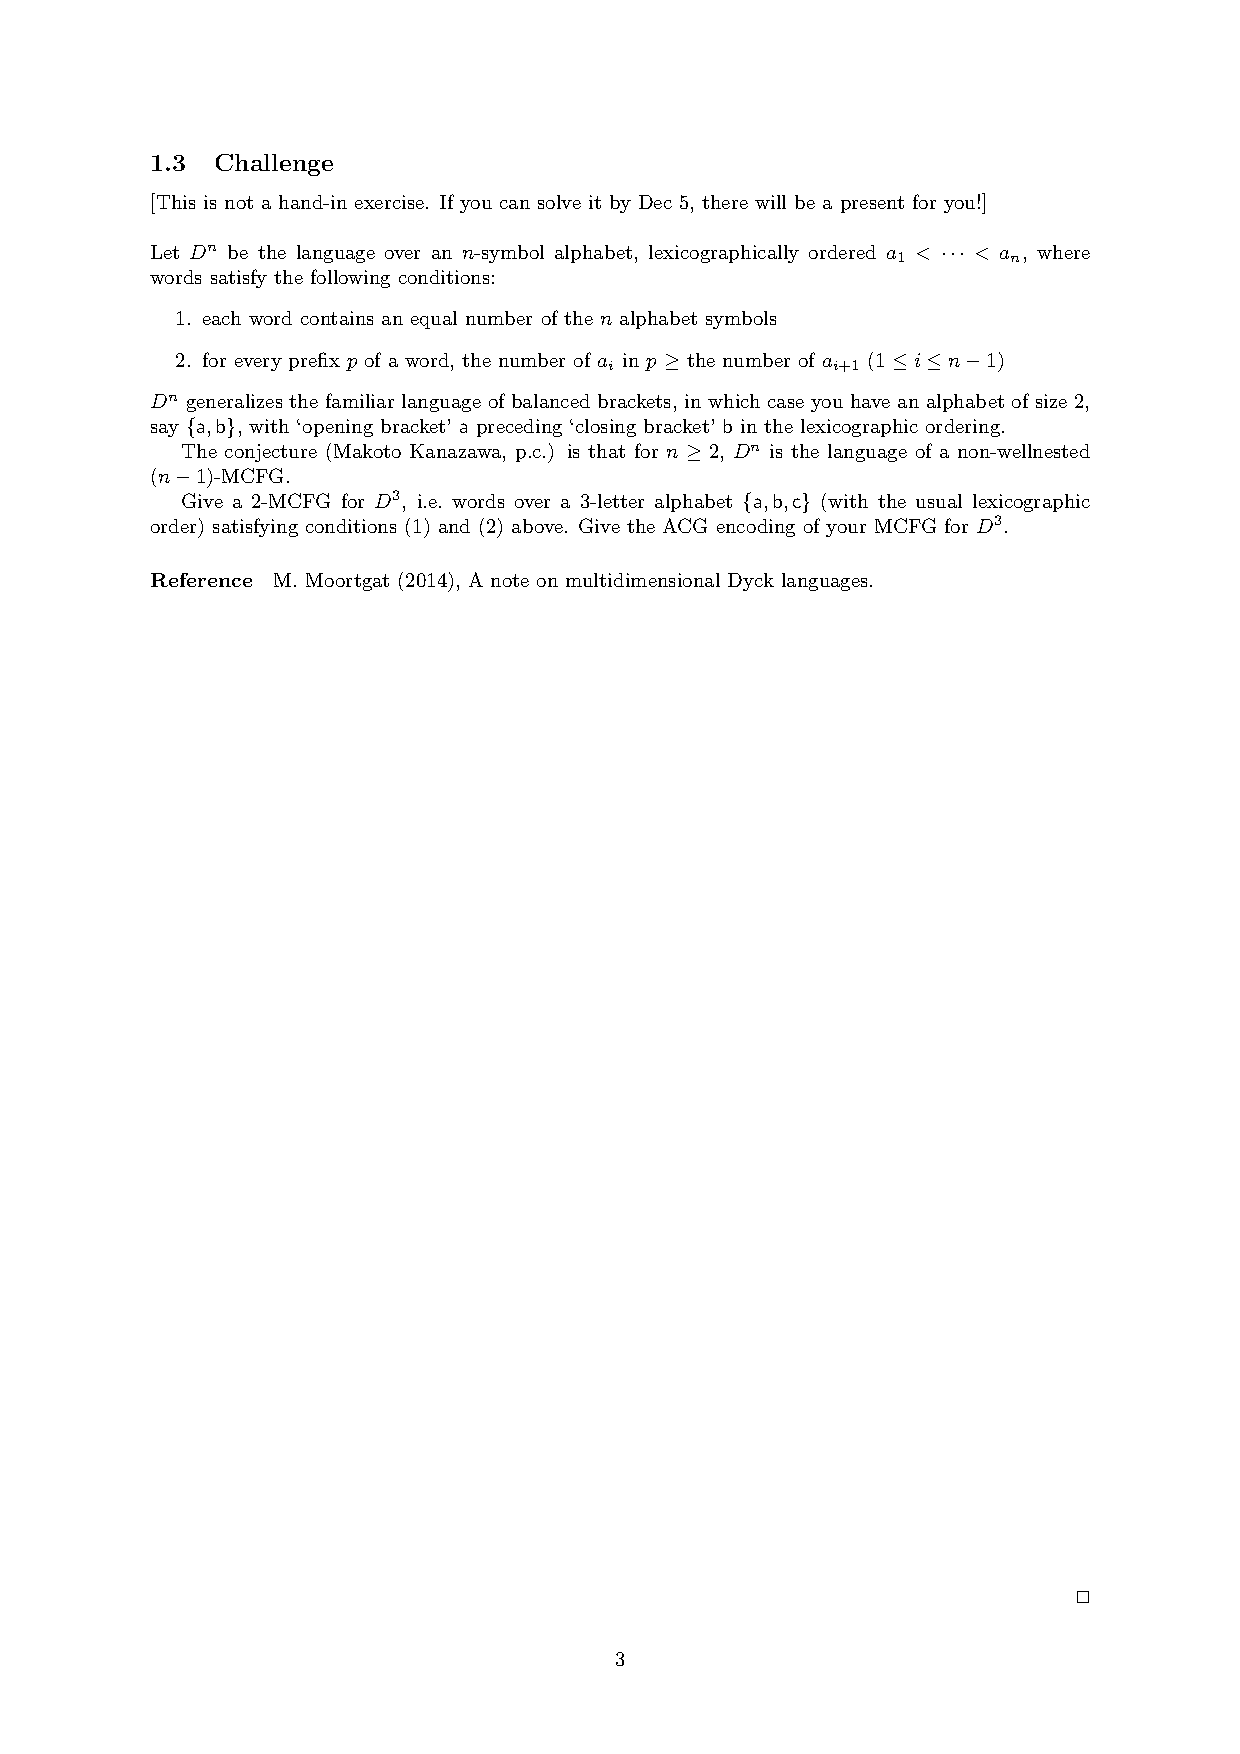
\includegraphics[clip, trim=1cm 18cm 1cm 1cm, scale=.55]{quiz.pdf}}
	\end{center}
	\end{frame}

%	\begin{frame}{}
%		\epigraph
%			{When you depart for Ithaca,\\wish for the road to be long,\\full of adventure, full of knowledge.}
%			{\textit{C. P. Cavafy\\ Ithaca}}
%	\end{frame}

	\begin{frame}{Some examples}
		\hspace{1cm}
		\begin{minipage}{.4\textwidth}
		\textsc{Dyck words}
		\begin{itemize}
			\item \textcolor{green}{abc}
			\item \textcolor{green}{aabbcc}
			\item \textcolor{green}{abcabcabacbc}
		\end{itemize}	
		\end{minipage}
		\pause
		\begin{minipage}{.4\textwidth}
		\textsc{Non-dyck words}
		\begin{itemize}
			\item \textcolor{red}{aabb}
			\pause
			\item \textcolor{red}{aabbbcc}
			\pause
			\item \textcolor{red}{abcacb}
		\end{itemize}	
		\end{minipage}
		\vspace{1cm}
		\pause
		\begin{figure}[h!]
		\centering
		
\begin{tikzpicture}[every node/.style={anchor=base},xscale=.25,yscale=.4]
			\node (n0) at (0,0) {$a$};
			\node (n1) at (1,0) {$b$};
			\node (n2) at (2,0) {$a$};
			\node (n3) at (3,0) {$b$};
			\node (n4) at (4,0) {$a$};
			\node (n5) at (5,0) {$c$};
			\node (n6) at (6,0) {$b$};
			\node (n7) at (7,0) {$c$};
			\node (n8) at (8,0) {$a$};
			\node (n9) at (9,0) {$b$};
			\node (n10) at (10,0) {$c$};
			\node (n11) at (11,0) {$c$};
			\pause
			\draw (n0) edge [rred, bend left=90] (n1);
			\draw (n1) edge [rred, bend right=90] (n5);
			\pause
			\draw (n2) edge [ggreen, bend left=90] (n3);
			\draw (n3) edge [ggreen, bend right=90] (n7);
			\pause
			\draw (n4) edge [bblue, bend left=90] (n6);
			\draw (n6) edge [bblue, bend right=90] (n10);
			\pause
			\draw (n8) edge [pyellow, bend left=90] (n9);
			\draw (n9) edge [pyellow, bend right=90] (n11);
		\end{tikzpicture}
		\caption*{First-match policy}
		\end{figure}
	\end{frame}
	
	\begin{frame}{Grammar of triple insertions}
		\begin{figure}[h!]
		\begin{align}
		\setcounter{equation}{0}
		\s{S}(xy) \leftarrow \s{W}(x,y)&. \\
		\s{W}(\epsilon, xy\textbf{abc}) \leftarrow \s{W}(x,y)&. \\
		\s{W}(\epsilon, x\textbf{a}y\textbf{bc}) \leftarrow \s{W}(x,y)&. \\
		...... \nonumber \\
		\setcounter{equation}{59}
		\s{W}(\textbf{ab}x\textbf{c}y, \epsilon) \leftarrow \s{W}(x,y)&. \\
		\s{W}(\textbf{abc}xy, \epsilon) \leftarrow \s{W}(x,y)&. \\
		\s{W}(\epsilon, \textbf{abc})&. \\
		\s{W}(\textbf{a}, \textbf{bc})&. \\
		\s{W}(\textbf{ab}, \textbf{c})&. \\
		\s{W}(\textbf{abc}, \epsilon)&.
		\end{align}
		\end{figure}
	\end{frame}
	
	\begin{frame}{Grammar of triple insertions}
		\begin{figure}[h!]
		\centering
		\begin{tikzpicture}[every node/.style={anchor=base}, every edge/.style={thick}]
			\node (n0) at (0,0) {$a$};
			\node (n1) at (1,0) {$a$};
			\node (n2) at (2,0) {$b$};
			\node (n3) at (3,0) {$b$};
			\node (n4) at (4,0) {$a$};
			\node (n5) at (5,0) {$c$};
			\node (n6) at (6,0) {$b$};
			\node (n7) at (7,0) {$a$};
			\node (n8) at (8,0) {$c$};
			\node (n9) at (9,0) {$c$};
			\node (n10) at (10,0) {$b$};
			\node (n11) at (11,0) {$c$};
			\pause
			\draw (n0) edge [rred, bend left=90] (n2);
			\draw (n2) edge [rred, bend right=90] (n5);
			\pause
			\draw (n1) edge [ggreen, bend left=90] (n3);
			\draw (n3) edge [ggreen, bend right=90] (n8);
			\pause
			\draw (n4) edge [bblue, bend left=90] (n6);
			\draw (n6) edge [bblue, bend right=90] (n9);
			\pause
			\draw (n7) edge [pyellow, bend left=90] (n10);
			\draw (n10) edge [pyellow, bend right=90] (n11);
		\end{tikzpicture}
		\caption*{Straddling counter-example}
		\end{figure}
	\end{frame}
	
	\begin{frame}{Overview}
    \begin{itemize}
      \item Background
      \item $G0$: Triple insertion
      \item Meta-grammar notation
      \item $G_0'$: Triple insertion (in $O_2$ notation)
      \item $G_1$: G0' + interleavings
      \item $G_2$: incomplete words
      \item $G_3$: G2 + 3-ins
      \item \alert{DEMO}: \textbf{dyck}
      \item Refined states
      \item Constraints (notation)
      \item ARIS
      \item Results
      \item Road to completeness
      \item Correspondences
      \item \alert{DEMO}: \textbf{dyckviz}
    \end{itemize}
	\end{frame}
  	
  	\begin{frame}{Theoretical background}
  	\end{frame}
  	\begin{frame}{Modelling techniques}
  	\end{frame}
  	\begin{frame}{Implemented grammars}
  	\end{frame}
  	\begin{frame}{Road to completeness}
  	\end{frame}
  	\begin{frame}{Tools}
  	\end{frame}
  	\begin{frame}{Demo}
  	\end{frame}
\end{document}